%Exemplo de capitulo

\chapter{Implementação e Experimentos}

Neste capítulo será apresentada uma implementação de um sistema de localização
de imagens de veículos e os resultados das medições de desempenho do mesmo.

Também será apresentado um breve histórico mostrando algumas abordagens que
foram tentadas antes da implementação final ter sido obtida, mostrando por que
elas falharam.

\section{Arquitetura Global}
Desde as primeiras tentativas de implementação algumas características do
software permaneceram sem alterações. Isso inclui o uso de um detector para
construir um localizador e a lista de módulos de software. Estas
características são as listadas nessa seção.

Redes neurais em geral requerem grande quantidade de exemplos de treinamento
para evitar overfitting \cite{hawkins2004problem}. É crucial para o
sucesso de uma implementação acesso a dados ou a capacidade de produzi-los.

\begin{figure}[!htb]
	\centering
	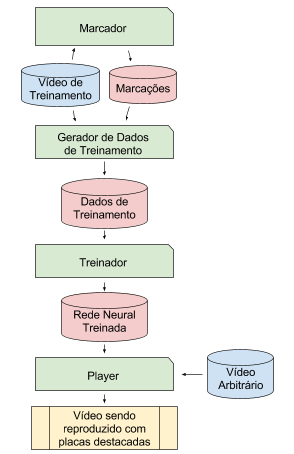
\includegraphics{cap5_arquit_global.png}
	\caption{Arquitetura Global da Implementação}
	\label{fig:cap5_arquit_global}
	Diagrama ilustrando os quatro componentes de software em verde, os vídeos
	de entrada em azul, as informações intermediárias em vermelho e a saída do
	sistema em amarelo (próprio autor).
\end{figure}

Em todas variações tentadas de implementação optou-se por gerar os dados de
treinamento. Para tal, dois softwares foram desenvolvidos: um software de
marcação manual de placas em vídeo e um software para geração desses dados.
Usando os dois softwares é possível gerar exemplos etiquetados em quantidade
suficiente no formato requerido pela rede neural. O treinamento e teste da rede
neural requereu o desenvolvimento de outros dois outros softwares. O primeiro
treina a rede neural, o segundo reproduz o vídeo enquanto aplica a rede neural
treinada, mostrando as placas identificadas. Isso resulta em quatro módulos de
software principais. O relacionamento entre eles é mostrado na figura
\ref{fig:cap5_arquit_global}.

A implementação de cada um destes módulos mudou durante a história do projeto,
porém as suas funções básicas permaneceram as mesmas.

\section{Abordagens Antiores}
Várias tentativas de foram feitas usando abordagens incorretas durante o
desenvolvimento do projeto. O software chegou a ser implementado por completo
três vezes, sendo que só produziu resultados satisfatórios na última.

A idéia inicial para este projeto era o uso de redes neurais não-convolucionais
aplicadas diretamente aos pixels das imagens. Para tal foi escolhida a
biblioteca neuroph, devido a familiaridade e ao uso da linguagem java. A
solução foi totalmente implementada conforme arquitetura ilustrada na figura
\ref{fig:cap5_arquit_global}.

Essa implementação usava imagens em tons de cinza e segmentos com dimensões HW
$32 \times 100$ aplicadas em uma rede neural totalmente conectada com 3200
entradas e uma saída. A segmentação era feita  usando stride de 100\%, ou
seja, dois segmentos vizinhos tinham o perímetro de um dos seus lados em comum.

Esta biblioteca foi logo descartada porque o tempo de treinamento era muito
longo, impedindo a busca eficiente de configuração das camadas ocultas que
gerasse o resultado desejado. Testes com topologias mais complexas, com maior
largura e profundidade nas camadas intermediárias, chegavam a passar de uma
semana de execução. Não houve nenhuma configuração encontrada com desempenho de
classificação remotamente aceitável.

Acreditando que seria possível resolver o problema encontrando os
hiperparâmetros corretos da rede neural, e sabendo que isso requeriria
múltiplos experimentos com topologias diferentes, adotou-se a biblioteca encog,
devido ao melhor desempenho de treinamento. Essa adaptação, requereu reescrever
boa parte código. Apesar do treinamento rodar quase a uma taxa de imagens 10
vezes maior que a biblioteca anterior, também não foi encontrada topologia
com com desempenho remotamente aceitável. A figura
\ref{fig:cap5_trein_redes_nao_conv} mostra a
evolução do treinamento para algumas sessões. Entre as listadas a que teve
melhor desempenho usava 3200 neurônios na camada de entrada, então 172, 137,
109, 87, 69, 55, 44, 35 e 28 neurônios nas camadas ocultas, terminando
com uma saída.

\begin{figure}[!htb]
	\centering
	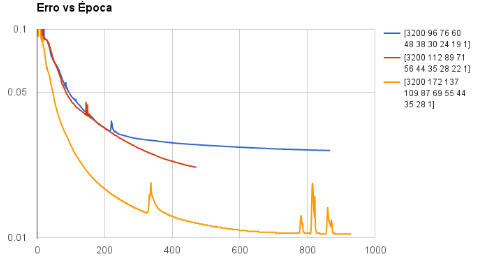
\includegraphics{cap5_trein_redes_nao_conv.png}
	\caption{Erro de treinamento de redes neurais não-convolucionais}
	\label{fig:cap5_trein_redes_nao_conv}
	A ordenada refere-se ao erro L2 calculado sem a raiz quadrada e suavizado
	usando exponential smoothing. A legenda refere-se ao número de neurônios
	em cada camada totalmente conectada.
\end{figure}


Quando o player era usado com as redes neurais resultantes desse treinamento o
resultado era muito ruim, com quantidade muito grande de falsos positivos.

O esquema de segmentação das imagens foi mudado de 100\% para 50\%, que é o
valor usado agora. A função que a rede neural modela foi modificada
várias vezes, mas
o resultado final, conforme visto no player, continuava ruim.

Após alguns meses a abordagem foi abandonada. Foi feita uma pesquisa sobre o
assunto descobriu-se a existência de redes neurais convolucionais. Infelizmente
a biblioteca encog e a neuroph não suportam este tipo de topologia. Também não
foram encontradas bibliotecas com grande base de usuários em java.

Neste ponto foi escolhida a biblioteca recém-lançada tensorflow. Inicialmente a
preparação dos dados de treinamento continuou sendo feita pelo código em java
que já havia sido escrito, enquanto o código de treinamento e execução foram
reescritos em python, por que era a única linguagem suportada quando essa
migração foi realizada.

O uso de duas linguagens de programação estava eliminando várias oportunidades
de reuso de código. Eventualmente o software de marcação e preparação de dados
de treinamento foi reescrito em python.

Desde os primeiros experimentos a abordagem usando redes neurais foi muito bem
sucedida.

\section{Escolha de Tecnologias}
A versão final da DCNN usa o framework TensorFlow do Google.
No TensorFlow usa-se a linguagem python para descrever um ou mais grafos onde
os nós são operações e as arestas são tensores. Uma vez que o grafo esteja
totalmente definido pode-se fornecer dados e solicitar o cálculo de qualquer
quantidade de nós. A execução em si ocorre em um runtime de alto desempenho
escrito em C++ e cuda, que pode ser distribuído entre múltiplas máquinas e pode
rodar em CPUs e GPUs.

A tecnologia foi escolhida por ser open source, e por ser a ferramenta
utilizada pelo Google. Esta biblioteca é fácil de usar para pequenos projetos,
como este, e poderosa para poder escalar para sistemas com múltiplos
computadores usando GPUs de alto desempenho. Portanto adquirir conhecimento
nesta tecnologia pode ser útil para projetos futuros.

O TensorFlow permite usar python 2 ou python 3. Eu optou-se por usar a versão 3
por que é a versão mais nova da linguagem, e é a versão padrão do sistema
operacional que uso para desenvolver os projetos.

Será usado OpenCV 3 e seu wrapper python para leitura e exibição do vídeo, para
algumas operações de manipulação de imagens e para gerar a interface com
usuário. O OpenCV tem primitivos suficientes para exibir uma janela contendo
uma imagem e capturar eventos de teclado e mouse. Isso é suficiente para toda a
interface gráfica.

Tanto o wrapper python do opencv quanto o TensorFlow representam dados
numéricos, como tensores, usando uma biblioteca numérica para python chamada
numpy. Ela será usada para várias operações, como extrair sub-imagens da frame
de vídeo que foi lida pelo opencv e fornecer estes dados para o TensorFlow.

Para representar as marcações que o usuário faz nos vídeos, para identificar
onde estão as placas, será usado o formato json. Este formato está se tornado o
padrão de facto para representação de dados no mercado. Além disso existem boas
bibliotecas em várias linguagens, inclusive python e java, que são minhas
linguagens principais.

O sistema operacional usado será Linux, particularmente a distribuição Arch
Linux. Eu já uso este sistema operacional no meu computador pessoal e do
escritório pelo seu sistema de atualização constante, que busca disponibilizar
o mais rápido possível as últimas versões de todos os seus componentes, como
kernel, compiladores, bibliotecas e softwares.
Arch Linux não é oficialmente suportado pelo projeto TensorFlow, mas existem
pacotes oferecidos pela comunidade tanto para versão estável quando para a
última versão git do projeto.
O servidor de código a ser usado é o git, por ser o padrão de facto do mercado.

Esse repositório já é usado pelo próprio projeto do TensorFlow.
Para edição de código será usado exclusivamente vim. Esse editor é sofisticado
e produtivo quando usado com uma linguagem como python.


\section{Recursos de Hardware}

O único recurso de hardware necessário é um computador. Como o treinamento de
redes neurais com imagens consome horas, possivelmente dias para cada sessão,
este computador idealmente seria um desktop de alto desempenho com pelo menos
uma placa de vídeo com suporte a tecnologia cuda.

Não foi possível ter acesso a computadores com a configuração recomendada.
Os computadores disponíveis durante a execução do projeto foram:

\begin{itemize}
\item Um notebook Core i7-3632QM com 4 cores (2 threads por core), 16 GiB
	de RAM;
\item Um notebook Core i5 com 2 cores (2 threads por core), 8 GiB de RAM,
	placa de video NVidia GT-750M com 2 GiB de RAM compatível com TensorFlow.
\end{itemize}

O desenvolvimento do projeto foi quase todo feito usando o Core i7. Assim que
o suporte a GPU foi incluída no código o notebook Core i5 começou a ser usado,
e, a partir deste ponto, ambos os coputadores passarm a ser usados.

\section{Implementação dos Módulos de Software}

Nesta seção está detalhada a implementação de cada módulo de software.

\subsection{Marcador}

\begin{figure}[!htb]
	\centering
	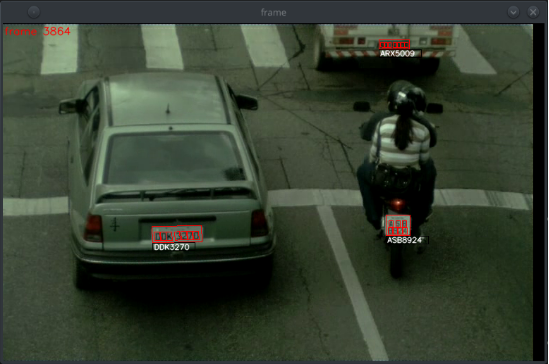
\includegraphics{cap5_tela_marcador.png}
	\caption{Interface com usuário do \emph{Marcador}}
	\label{fig:cap5_tela_marcador}
	A tela está mostrando 3 veículos marcados (próprio autor).
\end{figure}

O software marcador foi construído como um script python que recebe o nome de
um arquivo de vídeo como parâmetro. Ele permite:

\begin{enumerate}
\item Reproduzir o vídeo;
\item Pausar a reprodução do vídeo
\item Avançar / voltar frame-a-frame;
\item Saltar para uma frame digitando-se o número dela;
\item Quando o vídeo está em pausa, permite clicar no vídeo para adicionar um
	marcador de placa;
\item Usar o teclado para mover, rotacionar e alterar o marcador, de forma que ele
	circule corretamente a placa sendo marcada;
\item Digitar o número da placa veicular
\end{enumerate}

Como pode ser visto na figura \ref{fig:cap5_tela_marcador}, o software
marcador permite marcar placas de
carros e motos, e é possível identificar o número da placa. Isto tem como
objetivo permitir que as mesmas marcações possam ser usadas futuramente para
fazer OCR das placas. As marcações são salvas em um arquivo \emph{json}.

Quando uma frame possui pelo menos uma placa veicular marcada todo o resto da
imagem vai ser considerado pelo software de treinamento como região sem placa.
Por isso, se uma placa for marcada em uma frame, deve-se marcar todas as
placas.

\begin{table}
	\center
	\caption{Arquivos de vídeo usados durante o desenvolvimento}
	\begin{tabular}{ccccc}
		\Xhline{6\arrayrulewidth}
		Vídeo & Resolução HW & FPS & Tamanho & Duração \\ [2mm]
		\Xhline{2\arrayrulewidth}
		video1.avi & 480x768 & 25,0 & 141 MiB & 8:27 \\ [2mm]
		video2.avi & 1080x1920 & 25,0 & 1,0 GiB & 36:16  \\ [2mm]
		video3.avi & 1080x1920 & 25,0 & 465 MiB & 8:02  \\ [2mm]
		\Xhline{6\arrayrulewidth}
	\end{tabular}
	\label{tbl:videos}
\end{table}

Todo o desenvolvimento foi feito usando três vídeos. As características dos
vídeos estão listadas na tabela \ref{tbl:videos}, e uma frame de cada vídeo
está mostrada na figura \ref{fig:cap5_3_videos}.

\begin{figure}[!htb]
	\centering
	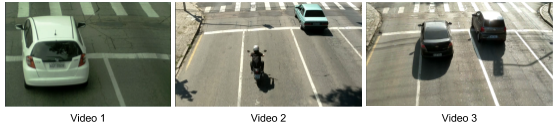
\includegraphics{cap5_3_videos.png}
	\caption{Uma frame de cada vídeo usado durante o desenvolvimento}
	\label{fig:cap5_3_videos}
	(próprio autor).
\end{figure}

A tabela \ref{tbl:marc_videos} mostra a quantidade de marcações feitas em cada
vídeo. A maior parte das marcações foram feitas no \emph{video1}.

\begin{table}
	\center
	\caption{Marcações feitas em cada vídeo}
	\renewcommand{\arraystretch}{1.5}
	\begin{tabular}{c c c}
		\Xhline{6\arrayrulewidth}
		\textbf{Vídeo} &
			\textbf{Quadros Marcados} &
			\textbf{Placas Marcadas} \\
		\Xhline{2\arrayrulewidth}
		video1.avi & 191 & 233 \\
		video2.avi & 71  & 71  \\
		video3.avi & 0   & 0   \\
		\Xhline{6\arrayrulewidth}
		TOTAL      & 262 & 304 \\
	\end{tabular}
	\label{tbl:marc_videos}
\end{table}


\subsection{Gerador de Dados de Treinamento}
\subsection{Treinador}
\subsection{Player}

\section{Experimentos e Desempenho}
